\documentclass{article}
\usepackage{CJKutf8}
\usepackage{graphicx}
\usepackage{color}
\begin{document}
\begin{CJK}{UTF8}{bkai}
\title{\Huge \color{blue} 聽歌辨識歌手  srs }
\author{第11組   李政憲 張哲郡 游登翔 劉彥麟 張友澤}
\maketitle
\begin{figure}[h]
\begin{center}
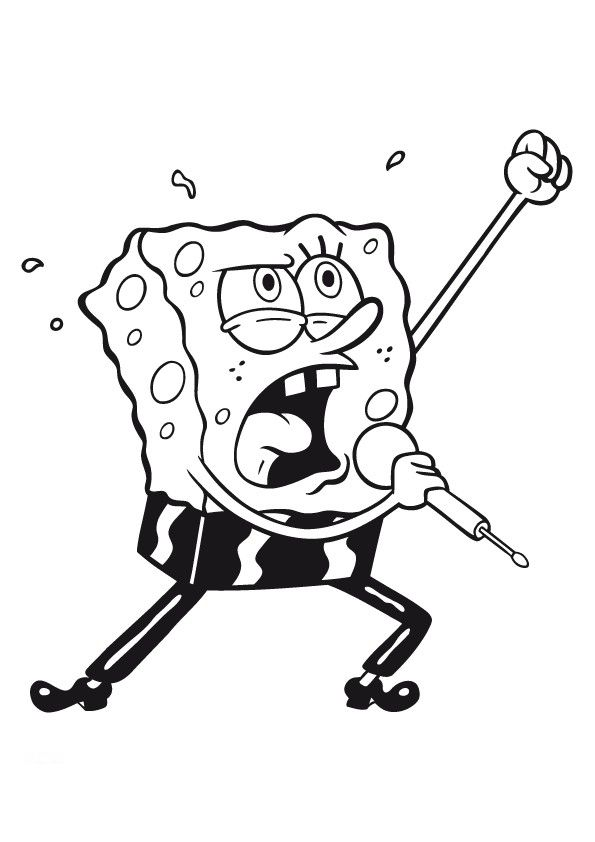
\includegraphics[width=8.5cm]{sing.jpg}
\end{center}
\label{fig:1}
\end{figure}
\newpage
\section{\huge \bf \color{blue}  introduction\\}

\subsection{\Large Purpose\\}
\large 做出一個只要輸入進去一首歌的音檔 就能判別出唱的歌手是誰的project
\subsection{\Large Intended Audience and Reading Suggestions\\}
\large intended Audience : 想要查詢自已聽到的歌是誰唱的的user \\\\
閱讀建議:對使用者而言要多注意"External interface"的部分\\
並且需要具備一定程式知識
\subsection{Project Scope\\}
這是個獨立的project, 
其目的為使user能辨識出聽到的歌是來自於哪位歌手

\newpage


\section{\huge\bf \color{blue}  Overall Description\\}

\subsection{\Large Product Perspective\\}
 \large 這個project利用很多首歌訓練出了各種歌手的特徵值 再利用這些特徵值辨別出我們輸入進去的是哪位歌手\\

\subsection{\Large Product Functions}
\large 輸入進去歌曲的音檔 就能讓它判斷是我們給的歌手們(分類)中的哪位\\

\subsection{\Large User Classes and Characteristics\\}
  \Large 聽線上電台的人, 實況的觀眾等等想知道當下聽到的歌是誰的歌的user\\\\%有時候會報錯,改成\newline
\begin{figure}[h]
\begin{center}
\includegraphics[width=11cm]{user.png}
\end{center}
\label{fig:1}
\end{figure}
\newpage
\subsection{\Large Operating Environment \\}
 \Large Operating system: Windows 10\\
platform:pycharm python3\\

\subsection{\Large Design and Implementation Constraints\\}
   \Large 因為大部分的歌都會有伴奏 \\
有些甚至快大過歌手本身的歌聲,\\
所以實際再辨別時是有難度的\\
音檔轉換為頻譜圖可能會失真\\
訓練用的MP3檔長度須為10秒
\subsection{\Large  Assumptions and Dependencies\\}
  \Large  這份專案是先假設即使沒有去除掉背景音\\
 電腦仍然能透過train來辨別出該歌手的特徵\\
並順利辨識\\
需先安裝:
音訊處理:ffmpeg\\
程式碼:keras tensorflow numpy sklearn
\newpage

\section{\huge\bf  \color{blue} External Interface Requirements\\}
\subsection{\Large User Interfaces\\}
\begin{figure}[h]
\begin{center}
\includegraphics[width=15cm]{ui.png}
\end{center}
\caption{為predict.py}
\label{fig:1}
\end{figure}
\subsection{\Large Hardware Interfaces\\}
CPU:intel i5-4570\\
RAM:16GB\\
x64型處理器\\
GPU:NVDIA GeForcee GT 640\\

\newpage
\subsection{\Large Software Interfaces\\}
operating system:x64位元作業系統 \\
 windows 10\\
python 3 IDE \\
影像處理:ffmpeg\\
\begin{figure}[h]
\begin{center}
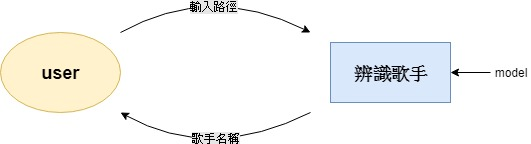
\includegraphics[width=13cm]{software_interface.jpg}
\end{center}
\label{fig:1}
\end{figure}
\newpage



\section{\huge\bf \color{blue}  System Features }
\subsection{\Large Description and Priority }
	
	透過機器學系對歌曲進行訓練,用訓練出的模型來判斷其他mp3檔的歌手名稱,優鮮度是以判斷正確為最高優先。
\begin{figure}[h]
\begin{center}
\includegraphics[width=14cm]{FS.jpg}
\end{center}
\caption{為系統流程圖}
\label{fig:2}
\end{figure}

\subsection{\Large Stimulus/Response Sequences}
	\begin{itemize}
		\item case1:觸擊save\_data:\\
			建立dataset裡各個歌手的.npy檔案
		\item case2:觸擊start\_train:\\
			生成由.npy黨所訓練的model
		\item case3:輸入正確路徑:\\
			回傳判斷個手名稱
		\item case4:輸入錯誤路徑:\\
			不回應
	\end{itemize} 
\subsection{ \Large Functional Requirements}
 \begin{center}
	\begin{tabular}{|c|p{3cm}|c|c|c|}\hline
		需求編號 &  需求描述&輸入&處理&輸出 \\ \hline
		FR001 &  新增歌手進入數據集&mp3檔&以mp3檔訓練 model&model \\ \hline
		FR002 &  辨識、預測歌手名稱&歌曲路徑&model判斷&歌手名稱\\\hline
	\end{tabular}
\end{center}

\section{\huge\bf  \color {blue}  Other Nonfunctional Requirements }
\subsection{ \Large Performance Requirements}
\begin{center}
	性能需求\\
	\begin{tabular}{|c|p{8cm}|}\hline
		需求編號 & 需求描述 \\ \hline
		PR001 &  一位歌手需50MB的容量  \\ \hline
		PR002 & 預測所需求時間1-5秒  \\ \hline
	\end{tabular}
\end{center}
\begin{center}
	易用需求\\
	\begin{tabular}{|c|p{8cm}|}\hline
		需求編號  & 需求描述 \\ \hline
		PR003  &介面簡單易於操作  \\ \hline
	\end{tabular}
\end{center}
\begin{center}
	環境需求\\
	\begin{tabular}{|c|p{8cm}|}\hline
		需求編號 & 需求描述 \\ \hline
		PR004 & 程式碼需相容Python3.0以上版本  \\ \hline
	\end{tabular}
\end{center}
\begin{center}
	操作需求\\
	\begin{tabular}{|c|p{8cm}|}\hline
		需求編號  & 需求描述 \\ \hline
		PR005  &訓練新歌手的mp3檔需200筆  \\ \hline
	\end{tabular}
\end{center}

\newpage
\Huge\bf   Thank you for watching


\end{CJK}
\end{document}
